\chapter{Landau Fermi Liquid Theory}

To begin with
\href{https://www.youtube.com/watch?v=2Z6UJbwxBZI}{Superfluid Helium}
on YouTube.

Stick stand straightly in a cup of liquid \ce{He}
$p \propto \pdv Sn \pdv nT$, i.e., entropy per particle, $\pdv nT \equiv \nabla n$ is the density graident.
Ref: Volovik, Universe in a drop of \ce{He}.

LFLT paradigim of many-theory. 1900, Onnes.
\begin{enumext}
  \item Adiabatic: quasi-particle concept weight, effective mass
  \item Variational $\xlongrightarrow{\braket<n>\to\delta\braket<n>}$ functional
  \item Quantum-statistical: Landau parameters
  \item Effective theory
  \item Collective: mode/excitation, zero sound; first sound $\pdv n/\mu$.
  \item $J^{-1}(\epsilon) \propto (\epsilon^2 + \pi^2T^2)$
  \item Degenerate Fermi gas of Sommerfeld
  \[
    \epsilon_k = \frac{k^2}{2m} - \mu
  \]
  let $k_f^2/2m = \mu$, then $n(\bm k) = \begin{cases}
  1, & |k| < k_f\\ 0, & |k| > k_f
  \end{cases}$

  \begin{tikzpicture}
    \draw [->] (-2,0) -- (2,0) node [below] {$k_x$};
    \draw [->] (0,-2) -- (0,2) node [right] {$k_y$};
    \filldraw [pattern = north west lines] (0,0) circle (1);
    \draw [->, thick] (0,0) -- (-45:1) node [right] {$k_f$};
  \end{tikzpicture}
  
  The density of states at Fermi energy (or Fermi surface along the circle in the Figure above)
  \begin{align}
    N(0) & = 2 \frac{(4\pi)p^2}{(2\pi\hbar)^3} \odv p{\epsilon_p}\bigg|_{p=p_f}
  = \frac{mp_f}{\pi^2\hbar^3}\\
    N(E) & = \int_{\epsilon_k = 0}^{\epsilon_k = \epsilon} \frac{\d\bm k}{(2\pi)^2} n(\bm k) = \int \d\epsilon \rho(\epsilon) n(\epsilon)
  \end{align}
  where $\rho(\epsilon)$ is the density of state. The total energy
  \begin{equation}
    E = \int \d\epsilon \rho(\epsilon) \epsilon n(\epsilon)
  \end{equation}
  Similarly, the heat capacity
  \begin{equation}
    C_v = \odv ET = \frac{\pi^3}{3} N(0) k_0^2\bigg|_{C_{v,T}\to 0} = \gamma
  \end{equation}
  $\pdv {C_v}/T\big|_{T\to0}$.
  The eexception $\chi_c = \pdv n/\mu$.
  \item magnetic susceptibility.
  
  When a magnetic field $\bm B$ is applied, we will get an energy diffenerce from spin-up and spin-down $\mu(N_\uparrow - N_\downarrow)\mu_BB$.
  The magnetic susceptibility
  \begin{equation}
    \chi = \mu_F(N_\uparrow - N_\downarrow)/B = \mu_F^2 N(0)
  \end{equation}
  $\mu_F = \mu_B = \frac{e\hbar}{2m}$. $\mathcal E(\epsilon, k, \cdots)$,
  $\mu_B(\epsilon, k, \cdots)$.
  The Wilson ratio
  \begin{equation}
    W = \frac\chi\gamma = 3\ab(\frac{\mu_F}{\pi k_B})^2
  \end{equation}
  $v_i = \frac{k^2}{2m} \approxeq \frac{2k_F\delta k}{2m}$, $m^* = (2.8) m_{(3\ce{He})}$, and the effect magnetic moment $(g^*)^2 = 3.3 (g^2)_{\ce{^3He}}$.
  $\epsilon(k) \sim m^*$.
\end{enumext}

The low energy excition of unperturbed Hamiltonian.
\begin{enumext}
  \item Quasi-particle $c_{p_0\sigma_0}^\dagger$:
  \[
    n_{p\sigma} = \begin{cases}
      1, & (p<p_f), $or$ p = p_0, \sigma = \sigma_0\\
      0, & $otherwise$
    \end{cases}
  \]
  \item Quasi-hole $c_{k_0\sigma_0}$:
  \[
    n_{p\sigma} = \begin{cases}
      1, & p<p_f $except$ p = p_0, \sigma = \sigma 0\\
      0, & $otherwise$
    \end{cases}
  \]
  \item Particle-hole pair (create one and annihilate one at the same time).
\end{enumext}
On the fermi surface,
\[
  [H, n_{pf,\sigma}] = 0 \quad (p_F \in \text{FS})
\]
If $p - p_F = \delta p$, then the function will linear to $\delta p$.
When taking the limit
\[
  [H, n_{pF,\sigma}] \propto \delta p \big|_{\delta p\to 0} \to 0
\]
Then, the expectation
\[
  \braket<\Psi_0|[H, n_p, \sigma]|\Psi_0 \propto \delta p|_{\delta\to p}>
\]
The residual scattering remains on the Fermi surface, which is forward scatting.
The two particles
\[
  (\bm p_1, \bm p_2) \to (\bm p_1 - \bm q, \bm p_2 + \bm q), \qq{and} q = 0
\]
form the restrict scattering phase space, $\operatorname{Mod}(\bm q) = 0$.
It is a narrow window, i.e., thine shell, near the fermi surface.

\section{Change-neutral Fermi Liquid (With short range interaction: $\mathsf{\sim 1/r^6}$)}

\[
  \delta n_{p\sigma} = n_{p\sigma} - n_{p\sigma}^{(0)}
\]
from equilibrium static
\[
  \begin{tikzpicture}[baseline]
    \draw [<->] (0,1) node [left] {\mbox{$n^0$}} -- (0,0) -- (1,0);
    \draw (0,.5) -- (.5,.5) -- (.5,0) node [below] {$k_x$};
  \end{tikzpicture}
  \longrightarrow
  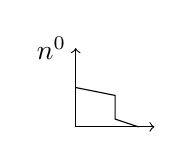
\begin{tikzpicture}[baseline]
    \draw [<->] (0,1) node [left] {\mbox{$n^0$}} -- (0,0) -- (1,0);
    \draw (0,.5) -- (.5,.4) -- (.5,.1) -- (.8,0);
  \end{tikzpicture}
\]
Then the functional equation
\begin{equation}
  E = E_0 + \sum_{p\sigma} (E_{p\sigma}^{(0) - \mu}) \delta n_{p\sigma}
    + \frac12 \sum_{pp'\sigma\sigma'} f_{p\sigma,p'\sigma'} \delta n_{p\sigma} \delta n_{p'\sigma'} + \cdots
\end{equation}
means that $\delta n_{p\sigma}(E_{q\sigma}^{(0)}, \mu) E_{p\sigma}^{(0)}(\delta n_{p\sigma},\cdots) f(\delta n_p, E_{p}^{(0)}, \cdots)$.
\begin{equation}
  \fdv E{n_{p\sigma}}\bigg|_{\delta n_{p'\sigma'=0}} = \epsilon_{p\sigma}^{(0)} = E_{p\sigma}^{(0)} - \mu, \quad
  v_f = \odv{\epsilon_p}p \bigg|_{p=p_f} = \frac{p_f}{m^*}, \qq{and}
  N^*(0) = \frac{m^*p_F}{\pi^2\hbar^3}
\end{equation}
Then, we can also the landau parameters as the second order perturbation
\begin{equation}
  f_{p\sigma, p'\sigma'}
= \fdv[2]E{n_{p\sigma},n_{p'\sigma'}} \bigg|_{\delta n_{p''\sigma''} = 0}
\end{equation}
From the functional equation, we can have
\[
  \fdv E{n_{p\sigma}} = \epsilon_{p\sigma}
= \epsilon_c \epsilon_{p\sigma}^{(0)}
+ \sum_{p'\sigma'} f_{p\sigma,p'\sigma'} \delta n_{p'\sigma'}
\]
then the entropy
\[
  S \approxeq -k_B \sum_{p,\sigma} \ab[n_{p\sigma}\ln n_{p\sigma}
    + (1 - n_{p\sigma} \ln(1 - n_{p\sigma}))]
\]
Just mathematically, no coherent term
\[
  \braket<n_pn_{p'}>_C = \braket<n_pn_{p'}> - \braket<n_p>\braket<n_{p'}>
\]
the really defiened $S = -\rho\ln\rho = f(\braket<n>, \braket<n^2>, \braket<n^3>, \cdots)$.

Combine the two quantities
\begin{multline}
  F(\{n_{p\sigma}\})
= E_0(\mu) + \sum_{p\sigma} \epsilon_{p\sigma}^{(0)} \delta n_{p\sigma}
+ \frac12 \sum_{pp'\sigma\sigma'}
  f_{pp'\sigma\sigma'} \delta n_{p\sigma} \delta n_{p'\sigma'}\\
+ k_BT \sum[n_{p\sigma} \ln n_{p\sigma}
          + (1 - n_{p\sigma}) \ln (1 - n_{p\sigma})],
\end{multline}
and $\delta F = 0$. The (Helmbotz) Free energy is
\[
  F = E - ST
\]
where
\[
  E = \int \d k n_k\epsilon_k, \quad N = \int \d k n_k, \qq{and} E_0 = \int \d k \theta(|k - k_F|) \epsilon_k
\]
Since $\delta n = n_k - \theta(k - k_f)$, and $n^0 = \theta$, then
\[
  \delta E = \int \d k \epsilon_k \delta n_k
\]
to do the variation $\delta n_k$
\[
  \delta n = \underbrace{\nu^{(0)}(k)}_{\to \delta p_f}
+ \sum \underbrace{\pdv{n^0}k}_{\delta(k - k_F) \sim \pdif k\theta}
  \nu_k^{(1)} + \frac12 \pdv{n^0}{k_i, k_j} \nu_{k_i,k_j}^{(2)}
+ \cdots
\]

\section{Landau Fermi Liquid Theory}

The energy can be written as
\begin{equation}
  E = E_0 + \sum \epsilon_{p\sigma}^{(0)} \delta n_{p\sigma}
      + \frac12 \sum_{pp'\sigma\sigma'} f_{p\sigma p'\sigma'}
        \delta n_{p\sigma} \delta n_{p'\sigma'}
\end{equation}
where $\epsilon_{p\sigma}^{(0)}$ is the functional derivation
\begin{equation}
  \epsilon_{p\sigma}^{(0)} = \fdv E{n_{p\sigma}} \bigg|_\text{1st order},
\end{equation}
with $|\bm p| = |p_F|$ and the heat capacity $C_v \propto N^*(i)$.
The Fermi velocity is defined of the Fermi surface
\begin{equation}
  v_F = \odv{\epsilon^{(0)}}p \bigg|_{P_F} = \frac{p_F}{m^*}
\end{equation}
In 2nd order theory, we get the actual physical particle energy
\begin{equation}
  \fdv E{n_{p\sigma}} \bigg|_\text{2st order} = \epsilon_{\rho\sigma}
= \delta \epsilon_{\rho\sigma}^{(0)}
+ \underbrace{\sum_{p\sigma} f_{p\sigma p'\sigma'} \delta n_{p'\sigma'}}_
  \text{Renormalization part}
\end{equation}
The free energy for the Fermi liquid
\begin{equation}
  F = E - TS[\{\delta n_{p\sigma}\}]
\end{equation}

\begin{example}
  Consider the Hamiltonian
  \[
    \mathcal H = \sum E_p n_{p\sigma} + \frac12 \sum V(q)
    c_{p-q\sigma}^\dagger c_{p'+q\sigma'}^\dagger
    c_{p'\sigma'} c_{p\sigma}
  \]
  Denote $\braket<\Psi|\mathcal H|\Psi>$, where
  $\ket|\Psi> = \ket|n_{p_1\sigma_1} n_{p_2\sigma_2} \cdots>$.
  Then, the energy
  \[
    E = \sum E_p n_{p\sigma} + \frac\lambda2 \sum V(q) \braket<\Psi|\cdots|\Psi>
  \]
  we can pair
  \begin{enumext}[columns = 2]
    \item $c_{p'+q\sigma'}^\dagger$ with $c_{p'\sigma'}$,
    then $p' + q$ with $p'$: $q = 0$.
    \item $c_{p-q\sigma}^\dagger$ with $c_{p\sigma}$,
    then $p - q$ with $p$: $q = 0$.
    \item $c_{p'+q\sigma'}^\dagger$ with $c_{p\sigma}$,
    then $p' + q = p$.
    \item $c_{p-q\sigma}^\dagger$ with $c_{p'\sigma'}$,
    then $p - q = p'$.
  \end{enumext}
  Then we will get
  \[
    (\delta_{q = 0} - \delta_{p-q,p'} \delta_{\sigma\sigma'})
    n_{p\sigma} n_{p'\sigma'}
  \]
  the energy will become
  \[
    E = \sum E_p n_{p\sigma}
  + \frac\lambda2 \sum (V(0) - V(p - p') \delta_{\sigma\sigma'})
    n_{p\sigma} n_{p\sigma'}
  \]
  with
  \[
    f_{p\sigma p'\sigma' = \lambda(V(0) - V(p - p') \delta_{\sigma\sigma'})}
  \]
  which is so-called the Fermion-Renormalization group.
  Ref: Shanker, RMP; or Polchinski on arXiv, EFT \& Fermi Surface.
\end{example}

\subsection{Feedback effects of interaction}

\begin{equation}
  \delta \epsilon_{p\sigma}^0 =
  \begin{cases*}
    -\delta \mu,              & isotropic enlarge / compression of Fermi surface\\
    -\sigma \mu_FB,           & magnetic field,\\
    \frac12m(\bm v - \bm u)^2,& shift in $\bm v$, in $\bm u$, the Galilean boost.
  \end{cases*}
\end{equation}
The actual physical particle energy
\begin{equation}
  \delta\epsilon_{p\sigma} = \delta\epsilon_{p\sigma}^{0}
+ \sum f_{p\sigma p'\sigma'} \delta n_{p'\sigma'}
\end{equation}
where
\[
  n_{p\sigma} = f(\epsilon_{p\sigma}^0 + \delta\epsilon_{p\sigma})
  \underset{T\to\sigma}\approxeq f(\epsilon_p^0)
+ f'(\epsilon_p^{(0)}) \delta\epsilon_{p\sigma}
= \underbrace{\theta(-\epsilon_p^0)}_{n_{p\sigma}^0} +
  \underbrace{[-\delta(\epsilon_p^0), \delta\epsilon_{p\sigma}]}_{\delta n_{p\sigma}}
\]
i.e., $n_{p\sigma} \to n_{p\sigma}^0$, and $\delta n_{p\sigma} \to \delta n_{p'\sigma'}$.
So, the actual physical particle energy can be written as
\[
  \delta \epsilon_{p\sigma} = \delta \epsilon_{p\sigma}^0 + \sum_{p'} f_{pp'} (-\delta(\epsilon_{p'}^0)) \cdot \delta \epsilon_{p'}
\]
where
\[
  f_{pp'} = \sum_l f_l P_l(\cos\theta), \quad 
  \delta \epsilon_p^{(0)} = v_l Y_{lm}(\theta,\phi), \quad
  \delta_{p\sigma} = \sum_l t_l Y_{lm}
\]
then, we obtain
\[
  t_l = v_l - F_l^s t_l = \frac{v_l}{1 + F_l^s}
\]
We shall only consider the leading term, i.e. effective mass per coleman
\[
  v_1 \propto \delta \epsilon_p^0 \approxeq - m\bm v_F \cdot \bm u = -m \cos\theta p_F
  \propto P_1(\cos\theta)
\]
Then, we have
\[
  t_1 = \frac{v_1}{1 + F_1^S}
\]
There will have a displacement of the fermi surface.

The effective mass satisfies
\[
  \odv\epsilon p = \frac{p_F}{m^*} = \frac{p_F}{m} + \frac{F_1^s p_F}{m^*}
\]
\begin{paracol}{2}
then, it can be expressed as
\[
  m^* = m(1 + F_1^s)
\]
V.s. the band effect mass,
\[
  m^* = m\ab(1 + \frac13 F_1^s)
\]
\switchcolumn \centering
\includegraphics[width = \linewidth]{image-1541}
\end{paracol}

\subsection{Equilibrium Properties}

We specific head
\begin{gather}
  \delta S = \frac1{TV} \sum(\epsilon_p - \mu) \delta n_p,\\
  C_V = S_1 = \frac{m^*p_F}{3\hbar^2} k_B^2T.
\end{gather}
E.Fradin. We can write
\begin{equation}
  \delta n_\sigma(T,\mu,\epsilon_p)
= \pdv n\epsilon [-(\epsilon_p -  \mu) \delta T + \delta \cancelto{\fdv ST}{\epsilon_p - \delta\mu}]
\end{equation}
Then, we have
\begin{multline}
  \delta S = -\frac1V \sum_p \pdv n\epsilon (\epsilon_p - \mu^2) \delta T
           = -\frac1V \underbrace{\int p^2 \odv p\epsilon}_\text{3D}
              \d\epsilon_p \pdv n\epsilon_p (\epsilon_p - \mu)^2 \delta T\\
= -k_B^2 N^*(0) \int \d x \pdv*[fun]{\frac1{\upe^x + 1}}x x^2 \delta T
\end{multline}
The Fermi energy for Landau Fermi liquid $E_F \propto T_F$, then
\begin{equation}
  T_F = \frac{p_F^2}{2m^*k_B} = \frac{\epsilon_F}{k_B}
\end{equation}
Then,
\begin{equation}
  \mu'(n, T) = -(\pdv Fn)_T = \mu(n,0)
- \frac{T_1^2}{4} k_s\ab(\frac13 + \frac n{m^*} \pdv{m^*}n) \frac{T^2}{T_F}
\end{equation}
The compressibility, $\delta \epsilon_p^{(0) = -\delta\mu}$. Then,
\begin{equation}
  \kappa = -\frac1V \pdv Vp = \frac1{n^2} \pdv n\mu
\end{equation}
which is so-called the charge susceplibility. Then,
\[
  \delta n_p = \pdv n{\epsilon_p} (\delta\epsilon_p - \delta\mu),
\]
where $\delta E_p = F_0^S \delta n_{p_F}$. Substitute it
\begin{equation}
  \delta n_p = -N(0) (F_D^s \delta n - \delta \mu)
\end{equation}
Then, we can obtain the relation between $\delta n$ and $\delta\mu$
\begin{equation}
  \fdv n\mu = \pdv n\mu = \frac{N(0)}{1 + F_0^s}.
\end{equation}
The Fermi sphere get smaller
\[
  \delta \epsilon_p^{(0)} = -\sigma \mu_F \beta
  \begin{cases}
    \delta \mu_h = + \frac B2,\\
    \delta \mu_l = - \frac B2,\\
  \end{cases}, \quad
  \pdv{S_Z}B = \frac{\delta n_\uparrow - \delta n_\downarrow}{B}, \quad
  \chi = \frac{\hbar^2}{2} \gamma^2 N(0) \frac{1}{1 + p_0^s}.
\]

\subsection{Thermodynamic stability of Fermi liquid}

\begin{equation}
  n_{p\sigma}^0 = \theta(p_F(0) - |\bm p|)
\end{equation}
Since the Gibbs free energy
\begin{equation}
  G = E - \mu n
\end{equation}
then
\begin{equation}
  (E - \mu_n) - (E - \mu_n)_0
= \frac1V \cancelto{\propto\delta p_F(\theta)}
    {\sum (\epsilon_p^0 - \mu) \delta n_p} +
  \frac1{2V^2} \sum f_{p\gamma'} \delta n_p \delta n_{p'}
\end{equation}
and
\begin{equation}
  \delta n_p = n_p - n_p^0 = \delta p_F \delta(p_F - |\bm p|)
- \frac12(\delta p_F)^2 \pdv*[fun]{(p_F - p)}p
\end{equation}
where
\[
  \delta p_F(\theta) = p_F(\theta) - p_F^0(\theta) \longrightarrow
  v_F\delta p_F(\theta) = \sum_{l=0}^\infty v_l P_l(\cos\theta)
\]
The 1st term
\[
  \delta - \mu \delta n = \sum \frac{N(0)}{(2l + 1) \delta}
  \ab[(v_{l\uparrow} + v_{l\downarrow})^2 \ab(1 + \frac{F_l^s}{2l + 1})
    + (v_{l\uparrow} - v_{l\downarrow})^2 \ab(1 + \frac{Fl^A}{2l + 1})].
\]
We should find the Fermi-stability condition
\begin{equation}
  \delta E - \mu\delta n > 0, \qq{and}
  1 + \frac{F_l^{S,A}}{2l + 1} \geq 0,
\end{equation}
and the Pometanchuk inequility (transition)
\begin{equation}
  F_l^{S,A} \geq -(2l + 1).
\end{equation}
If $p$-inequility, violated, then $\delta p_F = v_{l_0}$, which
will change the Fermi surface shape.

\subsection{Non-Equilibrium Properties}

Steady state

\subsection{Changed Fermi liquid: Landau-Silin theory}

$\delta n_p(x)$:
\begin{equation}
  \nabla^2 \phi_p = \frac e{\epsilon^0} \sum_{p'} \delta n_p (x)
= \frac{e}{\epsilon^0} \delta n(x)
\end{equation}
We can have
\begin{equation}
  \epsilon_{p\sigma}(x) = \epsilon_p^{(0)} + e\phi_p
+ \sum_{p'\sigma'} f_{p\sigma p'\sigma'} \delta n_{p'} (x)
\end{equation}
Then, take the Fourier transform
\begin{equation}
  \delta \epsilon_{p\sigma}(q) = e\phi_p(q)
+ \sum_{p'\sigma'} f_{p\sigma p'\sigma'}
  \underbrace{\delta n_{p'\sigma'}(\epsilon)}_{\delta n(\delta\epsilon_p)}
= \sum_{p'\sigma'} \ab(\frac{e^2}{\epsilon_0q^2}
+ f_{p\sigma p'\sigma'}) \delta n_{p'\sigma'}(q)
\end{equation}
where
\[
  \tilde f_{p\sigma p'\sigma'}(q) = \frac{e^2}{\epsilon_0q^2} + f_{p\sigma p'\sigma'}
= \frac{N^*(0)}{1 + \ab(\frac{e^2N^*(0)}{\epsilon_0q^2} + F_0^s)}
\equiv \chi_c(q) \propto \pdv n\mu
\]
where we can approximately write
\[
  1 + \ab(\frac{e^2N^*(0)}{\epsilon_0q^2} + F_0^s) \propto 1 + \frac{\kappa^2}{q^2}
\]
with $q \to 0$.
Then,
\[
  \delta \mu = \delta\mu \cdot\delta(x)9, \qq{the Foruier Transform}
  \delta n(x - x_0) = \mathcal F(\delta n(q)) \to \delta n(x) \delta n(x_0)
  \sim -\kappa \upe^{-\kappa|x - x_0|}
\]
where
\[
  \kappa \approxeq \frac{e^2 N^*(0)}{\epsilon_0} \frac12\ab(1 + F_0^S)
\]
The above is the so-called Thomas-Fermi screening.

Consider the quasi-particle length scale
\begin{equation}
  l \gg \frac{\hbar}{\Delta p} \sim \frac{\hbar v_F}{k_BT}
\end{equation}
$\delta n_p(x)$ is the Wigner distribution function,
where $p \to \braket<p>$ and $x \to \braket<x>$.
The wavepacket of $\delta n_p$
\begin{equation}
  W(\bm r_1, \sigma_1; \bm r_1, \sigma_2) =
  \int \d\bm p_1^3 \d\bm p_2^3
  \upe^{\iu/\hbar (\bm p_1\bm r_1 - \bm p_2\bm r_2)}
  \braket<a_{p_2\sigma_2}^\dagger(t) a_{p_1\sigma_1}(t)>
\end{equation}
The wave function of $q$ and $p$: $U^\dagger c_{p\sigma}^\dagger U$.
Ref: Fradkin's.

\subsection{Kinetic equation}

\begin{equation}
  \odv*{\delta n_{p\sigma}(\bm r, t)}t = 0
\end{equation}
where
\[
  [\delta n_{p = p_F}, H] = 0, \qq{and} [\delta n_{p \neq p_F}, H] \neq 0
\]
Then, q.p. will decay \textrightarrow\ q.p. collision, cause the quasi-particle lifetime
\[
  p_1 \leftrightarrow p_2: p_3,\ p_4.
\]
If we take the collisionless limit, then only achievable of $T = 0$.
Then term $I(\delta n_{p'})$, the collision integral, will describe the process
of quasi-particle lifetime.

The derivatives
\begin{align*}
  \odv*{\delta n_{\bm p}(\bm r,t)}t &
= \pdv*{\delta n}t + \pdv*{\ab(\odv{\bm r}t \delta n_{\bm p} (\bm r,t))}{\bm r}
+ \pdv*{\odv{\bm p}t \delta n_{\bm p}(\bm r, t)}{\bm p},\\
  \odv{\bm r_p}t & = \bm v_{\bm p} = \pdv{\epsilon_{\bm p}(\bm r, t)}{\bm p},\\
  \odv{\bm p}t & = \bm f_{\bm p}(\bm r, t)
= -\pdv*{\epsilon_p (\bm r, t)}{\bm r}
\end{align*}
Then, the Landau's kinetic equation becomes
\begin{equation}
  \pdv*{\delta n_{\bm p}(\bm r, t)}t
- \{\epsilon_{\bm p}(\bm r,t), \delta n_{\bm p}(\bm r,t)\} =
  \begin{cases*}
    0, & $T \to 0$,\\
    T(\delta n_{p'}), & $T$ is finite
  \end{cases*}
\end{equation}
where the Poisson brackets
\[
  \{\epsilon_p, \delta n_p\}_\text{PB}
= \pdv*{\epsilon_p \cdot \pdv*{\delta n_p}{\bm p}}{\bm r}
- \pdv{\epsilon_p}{\bm p} \cdot \pdv{\delta n_p}{\bm r}
\]
The external potential $U(\bm r, t)$ satisfies
\[
  \int \d\bm r U(\bm r, t) \delta n_{\bm p}(\bm r, t)
\]
Then, the derivative becomes
\[
  \pdv{\epsilon_{\bm r}}{\bm r} = \pdv U{\bm r}
+ \int \frac{\d^3\bm p'}{(2\pi\hbar)^3} f_{pp'} \pdv*{\delta n_p(\bm r, t)}{\bm r}
\]
To linearize this equation: keep to the 1st order derivative in $\bm r$
\[
  \odv*{\delta n}t = \pdv*{\delta n}t + \pdv*{(\bm v_p \cdot \delta n)}{\bm r}
                   + \pdv*{-\pdv{\epsilon}{\bm r} \cdot \delta n}p = 0
\]
where $\epsilon = \epsilon^0 + \delta \epsilon$, and the term
\[
  \pdv{\epsilon}{\bm r} \cdot \delta n \sim
  \pdv{\delta\epsilon}{\bm r} \cdot \pdv*{\delta\bm n}{\bm p}
\]
where $\pdv*{\pdv\epsilon p}\epsilon \delta$ the first derivative act on $\delta n$.
Then $\odv*{\delta n}t$ satisfies
\[
  \pdv*{\delta n}t + \bm v_p \pdv*{\delta n - \pdv*{n_p^0}\epsilon \delta \epsilon_p}{\bm r}
= \begin{cases}
  0,\\T(\delta n)
\end{cases}
\]
Apply the Foruier transformation to $t\upe^x \Rightarrow \omega,\ q$
\[
  (\omega - \bm q, \bm v_{\bm p}) \delta n_{\bm p}(\bm q, \omega) -
  \bm q, \bm v_{\bm p} \pdv{n^0}{\epsilon_p} \delta \epsilon_p (\bm q, \omega)
= \begin{cases}
  0, \\
  \end{cases}
\]
The conservation laws
\[
  n(\bm r, t) = \int \d^3\bm p n_p(\bm r, t)
\]
Since $\int \d^3\bm p[t, n_{p'}] = 0$,
$\int \d p \pdv*{[f_p, n_p]}{p} = 0$,
and the continuity equation
\[
  \pdv*{n(\bm r, t)}t + \nabla \cdot \bm j = 0
\]
then we have
\begin{equation}
  \bm j = \sum_{p, \sigma} \bm v_{\bm p} \cdot n_{\bm p, \sigma}
= \sum \nabla_p \epsilon_p \cdot n_p
\end{equation}
The energy conservation law (thermal transport $\Delta U(\bm r, t)$)
\begin{equation}
  \pdv*[fun]{E - Un}t - \nabla \bm j_F = -\bm j \cdot \nabla \bm u
\end{equation}
Then, we have
\[
  \bm j_E = \int \d p \nabla_r \epsilon_p (\bm r, t) (\epsilon_p - U) n_{p\sigma}
\]
and also the graident energy.

\section{Collective modes: zero sound}

\[
  \delta n_p(\bm r, t) = \sum_q \delta n_p(q, \omega)
  \upe^{\iu(\bm q \cdot \bm r-\omega t)}
\]
and the potential
\[
  U(\bm r, t) = U\upe^{\iu(\bm q\cdot\bm r-\omega t)}
\]
The frequency satisfies
\begin{equation}
  (\omega - \bm q \cdot \bm v_{\bm p}) \delta n_p(q, \omega)
+ \pdv{n_p^0}{\epsilon_p} \bm q \cdot \bm v_p
  (u + \int \d p' f_{pp'} \delta n_{p'} (q, \omega)) = 0
\end{equation}
where
\[
  \delta n_{\bm p} = -\pdv{n_p}{\epsilon_p} v_{\bm p}, \qq{and}
  v_{\bm p} = \sum_{l=0}^\infty v_l P_l(\cos\theta)
\]
Substitute them
\[
  v_p + \frac{\bm q \cdot \bm v_p}{\omega - \bm q \cdot \bm v_{\bm p}}
  \int \d p' f_{pp'} \pdv{n^0}{\epsilon_{\bm p}}
= \frac{\bm q \cdot \bm v_p}{\omega - \bm q \cdot \bm U_{\bm p}}U
\]
Then, we have the single frequency
\[
  S = \frac{\omega}{qv_F}, \qq{and}
  \Omega_{ll'}(S) = \frac12 \int_{-1}^1 \d x P_l(x) \frac{x}{x - S} P_{l'}(x)
\]
To diagonal $l$
\[
  \frac{v_l}{2l + 1} + \sum_{l'=0}^\infty \Omega_{ll'} F_{l'}^s \frac{v_{l'}}{2l' + 1}
= -\Omega-{l_0}U
\]
take $l' = l = 0$
\[
  \Omega_{00} = 1 + \frac S2 \ln\ab|\frac{S - 1}{S + 1}|
+ \iu\frac\pi2 S\theta(1 - |S|).
\]
When $S$ is small, we will omit the imaginary part
\[
  v_0(s) = -\frac{\Omega_{00}(s)U}{1 + F_0^S\Omega_{00}(S)}
\]
Take $0 \leq S < 1$ (1t sound damped), then
\[
  V_0(S) \to \delta n_p(x, t) \sim \delta n_p^{S_0}(x,t) \propto \upe^{-S},
\]
which is the so-salled $p-n$-continuity.
When $S > 1$,
\[
  1 + F_0^{(S)} \Omega_{00}(S_0) = 0, \qq{zero sound}
\]
means that the Fermit liquid self is resonatiny with external driving force,
corresponding to an collective eigenmode,
and there is none dissipative in the collisonless limit.

The frequency $S_0 = \frac{\omega_0}{q v_F}$, i.e.,
the disspresion relation of the collective eigenmode.